\documentclass[11pt,a4paper]{article}

\usepackage[margin=1in]{geometry}
\usepackage{mathptmx}
\usepackage{amsmath}
\usepackage{amssymb}
\usepackage{amsthm}
\usepackage{braket}
\usepackage{tikz}
\usepackage{quantikz}
\usepackage{enumitem}
\usepackage{hyperref}
\usepackage{xcolor}

\definecolor{circuitblue}{RGB}{40,80,160}

\hypersetup{
    colorlinks=true,
    linkcolor=circuitblue,
    urlcolor=circuitblue,
    citecolor=circuitblue
}

\theoremstyle{definition}
\newtheorem{definition}{Definition}[section]
\newtheorem{example}{Example}[section]
\newtheorem{theorem}{Theorem}[section]

\theoremstyle{remark}
\newtheorem*{intuition}{Intuition}
\newtheorem*{keypoint}{Key Point}

\pagestyle{plain}

\setlength{\parindent}{0pt}
\setlength{\parskip}{6pt}

\begin{document}

\begin{center}
    {\LARGE \textbf{Quantum Boltzmann Machines and QGANs}}\\[8pt]
    {\large QML}\\[12pt]
    \hrule
\end{center}

\vspace{12pt}
\tableofcontents
\newpage

%% ========================================================
\section{Overview}
%% ========================================================

so far in this course we've mostly focused on discriminative models --- classifiers, regressors, stuff that maps inputs to outputs. but some of the most exciting ML is generative: learning to \emph{produce} new data that looks like ur training set. think GANs generating faces, or Boltzmann machines learning probability distributions.

this lecture we dive into the quantum versions of these generative models. specifically: quantum Boltzmann machines (QBMs), quantum GANs (QGANs), and Born machines. these r genuinely cool bcs they exploit quantum mechanics in a deep way --- quantum superposition gives u access to exponentially large probability distributions that would be hard to represent classically.

the roadmap: first well recap the classical versions (Boltzmann machines and GANs), then quantize them, then discuss the key papers (zoufal et al. 2019 is the big one for QGANs), and finally look at applications and challenges.

fair warning: generative quantum models r still pretty experimental. training is hard, hardware is noisy, and the advantage question is open. but the ideas r beautiful, and some of the applications (loading distributions for quantum Monte Carlo, drug molecule generation) r genuinely promising.

%% ========================================================
\section{Classical Boltzmann Machines Recap}
%% ========================================================

before we quantize anything, lets make sure the classical foundations r solid.

\subsection{Energy-Based Models}

\begin{definition}[Energy-Based Model]
an energy-based model assigns an energy $E(\mathbf{x})$ to each configuration $\mathbf{x}$ of binary variables. the probability of a configuration is given by the Boltzmann distribution:
\[
p(\mathbf{x}) = \frac{e^{-E(\mathbf{x})}}{Z}, \quad Z = \sum_{\mathbf{x}} e^{-E(\mathbf{x})}
\]
where $Z$ is the partition function (normalization constant).
\end{definition}

\begin{intuition}
low energy = high probability. the model learns to assign low energy to configurations that look like training data, and high energy to everything else. its like a landscape where the training data sits in valleys.
\end{intuition}

for a general Boltzmann machine with visible units $\mathbf{v}$ and hidden units $\mathbf{h}$, the energy is:
\[
E(\mathbf{v}, \mathbf{h}) = -\sum_{i} a_i v_i - \sum_{j} b_j h_j - \sum_{i,j} W_{ij} v_i h_j - \sum_{i<i'} L_{ii'} v_i v_{i'} - \sum_{j<j'} M_{jj'} h_j h_{j'}
\]

where $a_i, b_j$ r biases, $W_{ij}$ r visible-hidden weights, and $L, M$ r intra-layer connections.

the marginal probability of the visible units is:
\[
p(\mathbf{v}) = \frac{1}{Z} \sum_{\mathbf{h}} e^{-E(\mathbf{v}, \mathbf{h})}
\]

this is wt we actually care about --- the distribution over things we can observe.

\subsection{Restricted Boltzmann Machines (RBMs)}

\begin{definition}[RBM]
a restricted Boltzmann machine is a Boltzmann machine where there r no intra-layer connections ($L = 0$, $M = 0$). visible units only connect to hidden units.
\end{definition}

the restriction is crucial bcs it makes the conditional distributions tractable:
\begin{align}
p(h_j = 1 | \mathbf{v}) &= \sigma\left(b_j + \sum_i W_{ij} v_i\right) \\
p(v_i = 1 | \mathbf{h}) &= \sigma\left(a_i + \sum_j W_{ij} h_j\right)
\end{align}
where $\sigma(x) = 1/(1 + e^{-x})$ is the sigmoid function.

the energy for an RBM simplifies to:
\[
E(\mathbf{v}, \mathbf{h}) = -\mathbf{a}^T \mathbf{v} - \mathbf{b}^T \mathbf{h} - \mathbf{v}^T W \mathbf{h}
\]

\begin{keypoint}
the RBM structure (bipartite graph, no intra-layer connections) is wt makes training feasible. without it, computing the gradient requires sampling from a distribution that has no nice factored form.
\end{keypoint}

\subsection{Contrastive Divergence Training}

training a Boltzmann machine means maximizing the log-likelihood:
\[
\mathcal{L} = \frac{1}{N} \sum_{n=1}^{N} \log p(\mathbf{v}^{(n)})
\]

the gradient has two terms (the ``positive'' and ``negative'' phases):
\[
\frac{\partial \mathcal{L}}{\partial W_{ij}} = \langle v_i h_j \rangle_{\text{data}} - \langle v_i h_j \rangle_{\text{model}}
\]

the positive phase $\langle \cdot \rangle_{\text{data}}$ is easy to compute bcs of the RBM structure: just clamp the visible units to training data and sample hidden units.

the negative phase $\langle \cdot \rangle_{\text{model}}$ requires sampling from the model distribution, which is hard. contrastive divergence (CD-$k$) approximates this by running only $k$ steps of Gibbs sampling:

\begin{enumerate}[label=\arabic*.]
    \item start from a training example $\mathbf{v}^{(0)}$
    \item sample $\mathbf{h}^{(0)} \sim p(\mathbf{h} | \mathbf{v}^{(0)})$
    \item sample $\mathbf{v}^{(1)} \sim p(\mathbf{v} | \mathbf{h}^{(0)})$
    \item repeat $k$ times
    \item approximate: $\langle v_i h_j \rangle_{\text{model}} \approx v_i^{(k)} \cdot p(h_j = 1 | \mathbf{v}^{(k)})$
\end{enumerate}

in practice, CD-1 (just one step) works surprisingly well. hinton showed this in 2002 and it made RBMs practical.

%% ========================================================
\section{Classical GANs Recap}
%% ========================================================

\subsection{The GAN Framework}

GANs (goodfellow et al. 2014) r a completely different approach to generative modeling.

\begin{definition}[GAN]
a generative adversarial network consists of two networks:
\begin{itemize}[nosep]
    \item \textbf{generator} $G$: takes random noise $\mathbf{z} \sim p_z$ and produces fake data $G(\mathbf{z})$
    \item \textbf{discriminator} $D$: takes data (real or fake) and outputs probability that its real
\end{itemize}
they r trained adversarially: $G$ tries to fool $D$, and $D$ tries to catch fakes.
\end{definition}

the minimax objective:
\[
\min_G \max_D \; V(G, D) = \mathbb{E}_{\mathbf{x} \sim p_{\text{data}}}[\log D(\mathbf{x})] + \mathbb{E}_{\mathbf{z} \sim p_z}[\log(1 - D(G(\mathbf{z})))]
\]

\begin{theorem}[Nash Equilibrium]
if $G$ and $D$ have unlimited capacity, the unique global optimum of the minimax game is:
\begin{enumerate}[nosep]
    \item the generator perfectly reproduces the data distribution: $p_G = p_{\text{data}}$
    \item the discriminator outputs $1/2$ everywhere (cant tell real from fake)
\end{enumerate}
at this equilibrium, $V(G^*, D^*) = -\log 4$.
\end{theorem}

\begin{intuition}
think of it as a counterfeiter ($G$) vs a detective ($D$). the counterfeiter keeps improving until the detective literally cant tell the difference. at Nash equilibrium, the counterfeits r perfect and the detective is just guessing.
\end{intuition}

\subsection{Training Dynamics}

in practice, we alternate gradient steps:
\begin{enumerate}[label=\arabic*.]
    \item \textbf{discriminator step}: fix $G$, update $D$ to maximize $V(G, D)$
    \item \textbf{generator step}: fix $D$, update $G$ to minimize $V(G, D)$
\end{enumerate}

the famous problem with GANs: training is unstable. u can get:
\begin{itemize}[nosep]
    \item \textbf{mode collapse}: $G$ produces only a few types of outputs instead of the full diversity
    \item \textbf{oscillations}: $G$ and $D$ chase each other without converging
    \item \textbf{vanishing gradients}: if $D$ is too good, $G$ gets no useful gradient signal
\end{itemize}

these problems dont go away when we go quantum --- tbh they sometimes get worse.

\subsection{Wasserstein Distance}

the Wasserstein GAN (WGAN) replaces the JS divergence with the Wasserstein-1 distance:
\[
W(p_{\text{data}}, p_G) = \sup_{\|f\|_L \leq 1} \left[ \mathbb{E}_{\mathbf{x} \sim p_{\text{data}}}[f(\mathbf{x})] - \mathbb{E}_{\mathbf{x} \sim p_G}[f(\mathbf{x})] \right]
\]

this gives smoother gradients and more stable training. the Wasserstein distance is particularly relevant for QGANs bcs it helps with the shot noise problem (more on this later).

%% ========================================================
\section{Quantum Boltzmann Machines}
%% ========================================================

now lets quantize. the key idea is simple: replace the classical energy function with a quantum Hamiltonian.

\subsection{From Classical to Quantum Energy}

\begin{definition}[Quantum Boltzmann Machine]
a quantum Boltzmann machine (QBM) is defined by a Hamiltonian $H$ acting on qubits. the model state is the thermal (Gibbs) state:
\[
\rho = \frac{e^{-\beta H}}{Z}, \quad Z = \mathrm{Tr}(e^{-\beta H})
\]
where $\beta$ is the inverse temperature.
\end{definition}

the crucial difference from classical: the Hamiltonian can contain non-commuting terms. a typical QBM Hamiltonian is:
\[
H = -\sum_{i} h_i Z_i - \sum_{i<j} J_{ij} Z_i Z_j - \sum_{i} \Gamma_i X_i
\]

the first two terms r just the classical Ising model (diagonal in the computational basis). the third term --- the transverse field --- is wt makes it quantum.

\begin{keypoint}
the transverse field terms $\Gamma_i X_i$ create quantum superpositions and entanglement in the thermal state. this means $\rho$ can represent correlations that no classical Boltzmann machine can efficiently represent. this is where the potential quantum advantage lives.
\end{keypoint}

\subsection{Quantum Thermal States}

lets be precise about wt the thermal state looks like. if we write $H$ in its eigenbasis:
\[
H = \sum_k E_k \ket{E_k}\bra{E_k}
\]
then:
\[
\rho = \frac{1}{Z} \sum_k e^{-\beta E_k} \ket{E_k}\bra{E_k}, \quad Z = \sum_k e^{-\beta E_k}
\]

for a purely classical Hamiltonian (only $Z_i$ terms), the eigenstates r computational basis states and $\rho$ is a diagonal density matrix --- just a classical probability distribution.

but when u add transverse field terms, the eigenstates r superpositions of computational basis states, and $\rho$ has off-diagonal elements (quantum coherences):

\begin{example}
single qubit with $H = -h Z - \Gamma X$:
\[
H = -\begin{pmatrix} h & \Gamma \\ \Gamma & -h \end{pmatrix}
\]
eigenvalues: $E_\pm = \mp \sqrt{h^2 + \Gamma^2}$

the thermal state has coherences between $\ket{0}$ and $\ket{1}$ --- its not just a mixture of up and down, but a genuine quantum state. the off-diagonal elements of $\rho$ in the computational basis r nonzero whenever $\Gamma \neq 0$.
\end{example}

\subsection{QBM Training}

to train a QBM, we want to maximize the quantum log-likelihood. if our training data consists of states $\{\sigma_n\}$, the log-likelihood is:
\[
\mathcal{L} = \frac{1}{N} \sum_{n=1}^{N} \mathrm{Tr}(\sigma_n \log \rho)
\]

equivalently, we can minimize the quantum relative entropy:
\[
S(\sigma \| \rho) = \mathrm{Tr}(\sigma \log \sigma) - \mathrm{Tr}(\sigma \log \rho)
\]

\begin{definition}[QBM Gradient]
the gradient of the log-likelihood with respect to a parameter $\theta_k$ (appearing in $H = \sum_k \theta_k O_k$) is:
\[
\frac{\partial \mathcal{L}}{\partial \theta_k} = \beta \left( \langle O_k \rangle_{\rho} - \langle O_k \rangle_{\sigma} \right)
\]
where $\langle O_k \rangle_{\rho} = \mathrm{Tr}(O_k \rho)$ is the expectation in the model state and $\langle O_k \rangle_{\sigma} = \mathrm{Tr}(O_k \sigma)$ is the expectation in the data state.
\end{definition}

this looks just like the classical case (positive phase minus negative phase), but theres a subtlety: when terms in $H$ dont commute, the gradient formula involves the Kubo-Mori inner product and things get more complicated. the formula above is exact only when all terms commute.

for the general non-commuting case, the exact gradient involves the integral:
\[
\frac{\partial \mathcal{L}}{\partial \theta_k} = \beta \int_0^1 \mathrm{Tr}\left(e^{-s\beta H} O_k e^{-(1-s)\beta H} \rho\right) ds - \beta \langle O_k \rangle_{\sigma}
\]

which is hard to compute. this is why approximate methods r important.

\subsection{Variational QBM (Zoufal et al.)}

\begin{keypoint}
the big practical problem with QBMs: preparing the thermal state $e^{-\beta H}/Z$ on a quantum computer is hard. u cant just ``cool down'' a quantum processor to the right temperature (well, u can on quantum annealers, but not on gate-based hardware).
\end{keypoint}

the variational approach: use a parameterized quantum circuit (PQC) to approximate the thermal state.

\begin{definition}[Variational QBM]
a variational QBM uses a PQC $U(\boldsymbol{\phi})$ to prepare an approximate thermal state. starting from a reference state $\ket{0}^{\otimes n}$:
\[
\rho(\boldsymbol{\phi}) = \mathrm{Tr}_A\left[U(\boldsymbol{\phi})\ket{0}\bra{0}^{\otimes (n+m)} U(\boldsymbol{\phi})^\dagger\right]
\]
where we trace out $m$ ancilla qubits to create a mixed state on $n$ system qubits.
\end{definition}

the training objective is to minimize:
\[
\mathcal{C}(\boldsymbol{\phi}) = S(\sigma_{\text{data}} \| \rho(\boldsymbol{\phi})) = -S(\sigma_{\text{data}}) - \mathrm{Tr}(\sigma_{\text{data}} \log \rho(\boldsymbol{\phi}))
\]

since $S(\sigma_{\text{data}})$ is constant, we just need to maximize $\mathrm{Tr}(\sigma_{\text{data}} \log \rho(\boldsymbol{\phi}))$.

this is still hard bcs computing $\log \rho$ is expensive. in practice, people use approximations like truncated Taylor series or variational bounds.

the circuit for a variational QBM typically looks like:

\begin{center}
\begin{quantikz}
\lstick{$\ket{0}$} & \gate{R_Y(\phi_1)} & \ctrl{1} & \gate{R_Y(\phi_5)} & \ctrl{1} & \meter{} \\
\lstick{$\ket{0}$} & \gate{R_Y(\phi_2)} & \targ{} & \gate{R_Y(\phi_6)} & \targ{} & \meter{} \\
\lstick{$\ket{0}$} & \gate{R_Y(\phi_3)} & \ctrl{1} & \gate{R_Y(\phi_7)} & \ctrl{1} & \trash{} \\
\lstick{$\ket{0}$} & \gate{R_Y(\phi_4)} & \targ{} & \gate{R_Y(\phi_8)} & \targ{} & \trash{}
\end{quantikz}
\end{center}

the top two qubits r ``visible'' (measured to get samples), the bottom two r ``ancilla'' (traced out to create a mixed state). the key insight: tracing out ancilla qubits from a pure entangled state creates a mixed state on the visible qubits, which can approximate a thermal state.

%% ========================================================
\section{Quantum GANs --- The Main Framework}
%% ========================================================

now for the main event. QGANs r arguably the most developed quantum generative model, thanks largely to zoufal et al. 2019.

\subsection{QGAN Architecture}

\begin{definition}[Quantum GAN]
a quantum GAN consists of:
\begin{itemize}[nosep]
    \item \textbf{quantum generator}: a PQC $G(\boldsymbol{\theta})$ that transforms an initial state (possibly with random input) into a quantum state encoding a probability distribution
    \item \textbf{discriminator}: either a classical neural network or a quantum circuit $D(\boldsymbol{\phi})$ that distinguishes real data from generated samples
\end{itemize}
\end{definition}

the most common setup (and the one zoufal et al. use):
\begin{itemize}[nosep]
    \item quantum generator with classical discriminator
    \item generator output is measured to produce classical samples
    \item discriminator is a standard neural network that takes these samples as input
\end{itemize}

\begin{intuition}
the quantum generator is like a quantum computer that outputs random numbers. but its not just any random numbers --- the PQC shapes the distribution so that the output statistics match the target distribution. the discriminator's job is to tell whether samples came from the real distribution or the quantum generator.
\end{intuition}

\subsection{QGAN Generator Circuit}

the generator circuit typically has this structure:

\begin{center}
\begin{quantikz}
\lstick{$\ket{0}$} & \gate{R_Y(\theta_1)} & \gate{R_Z(\theta_5)} & \ctrl{1} & \qw & \gate{R_Y(\theta_9)} & \gate{R_Z(\theta_{13})} & \ctrl{1} & \qw & \meter{} \\
\lstick{$\ket{0}$} & \gate{R_Y(\theta_2)} & \gate{R_Z(\theta_6)} & \targ{} & \ctrl{1} & \gate{R_Y(\theta_{10})} & \gate{R_Z(\theta_{14})} & \targ{} & \ctrl{1} & \meter{} \\
\lstick{$\ket{0}$} & \gate{R_Y(\theta_3)} & \gate{R_Z(\theta_7)} & \ctrl{1} & \targ{} & \gate{R_Y(\theta_{11})} & \gate{R_Z(\theta_{15})} & \ctrl{1} & \targ{} & \meter{} \\
\lstick{$\ket{0}$} & \gate{R_Y(\theta_4)} & \gate{R_Z(\theta_8)} & \targ{} & \qw & \gate{R_Y(\theta_{12})} & \gate{R_Z(\theta_{16})} & \targ{} & \qw & \meter{}
\end{quantikz}
\end{center}

this circuit has:
\begin{itemize}[nosep]
    \item $n = 4$ qubits, so it can represent distributions over $2^4 = 16$ values
    \item single-qubit rotation layers ($R_Y$, $R_Z$) for expressivity
    \item CNOT entangling layers for creating correlations
    \item two ``layers'' (repetitions of the rotation + entangling pattern)
    \item measurements in the computational basis to produce samples
\end{itemize}

the output probability distribution is:
\[
p_G(x) = |\braket{x | U(\boldsymbol{\theta}) | 0^n}|^2, \quad x \in \{0, 1, \ldots, 2^n - 1\}
\]

with $n$ qubits, we can represent distributions over $2^n$ outcomes using only $O(\text{poly}(n))$ parameters. this exponential compression is the key potential advantage.

\subsection{Noise Input for QGANs}

in classical GANs, the generator takes a random noise vector $\mathbf{z}$ as input. for QGANs, there r several approaches to incorporating randomness:

\begin{enumerate}[label=\arabic*.]
    \item \textbf{inherent quantum randomness}: just measure the output of the PQC. quantum mechanics provides the randomness ``for free'' through the Born rule. this is the most common approach.

    \item \textbf{random initial rotations}: apply random single-qubit rotations before the trainable circuit. the angles r sampled from some distribution each time.

    \item \textbf{ancilla-based}: use additional qubits in a fixed superposition state and trace them out.
\end{enumerate}

most QGAN implementations use approach 1 --- the quantum randomness from measurement is sufficient.

%% ========================================================
\section{Training QGANs}
%% ========================================================

\subsection{The Quantum Minimax Game}

the QGAN training objective mirrors the classical GAN:
\[
\min_{\boldsymbol{\theta}} \max_{\boldsymbol{\phi}} \; V(\boldsymbol{\theta}, \boldsymbol{\phi}) = \mathbb{E}_{x \sim p_{\text{real}}}[\log D_{\boldsymbol{\phi}}(x)] + \mathbb{E}_{x \sim p_{G_{\boldsymbol{\theta}}}}[\log(1 - D_{\boldsymbol{\phi}}(x))]
\]

the key difference: $p_{G_{\boldsymbol{\theta}}}$ comes from measuring a quantum circuit, so the gradients with respect to $\boldsymbol{\theta}$ involve quantum parameter-shift rules (which we covered in lecture 10).

\subsection{Alternating Optimization}

the training loop:

\begin{enumerate}[label=\textbf{Step \arabic*:}]
    \item \textbf{sample from generator}: run the quantum circuit $G(\boldsymbol{\theta})$ many times, measure to get samples $\{x_{\text{gen}}^{(1)}, \ldots, x_{\text{gen}}^{(M)}\}$

    \item \textbf{update discriminator}: using real samples and generated samples, update $\boldsymbol{\phi}$ to maximize $V$. this is classical optimization (backprop if $D$ is a neural network).

    \item \textbf{update generator}: using the discriminator's feedback, update $\boldsymbol{\theta}$ to minimize $V$. this uses the parameter-shift rule:
    \[
    \frac{\partial V}{\partial \theta_k} = \frac{V(\theta_k + \pi/2) - V(\theta_k - \pi/2)}{2}
    \]

    \item \textbf{repeat} until convergence (or until u lose patience --- QGAN training can be slow).
\end{enumerate}

\begin{keypoint}
each evaluation of the generator requires running the quantum circuit many times (shots) to estimate probabilities. with current hardware, this is the bottleneck. u need enough shots for good probability estimates, but each shot takes time on real hardware.
\end{keypoint}

\subsection{Loss Functions for QGANs}

besides the standard GAN loss (based on JS divergence), several alternatives have been explored:

\textbf{1. JS divergence (standard GAN):}
\[
\text{JS}(p_{\text{real}} \| p_G) = \frac{1}{2} \text{KL}(p_{\text{real}} \| m) + \frac{1}{2} \text{KL}(p_G \| m), \quad m = \frac{p_{\text{real}} + p_G}{2}
\]

\textbf{2. Wasserstein distance:}
\[
W_1(p_{\text{real}}, p_G) = \inf_{\gamma \in \Pi(p_{\text{real}}, p_G)} \mathbb{E}_{(x,y) \sim \gamma}[\|x - y\|]
\]

this is particularly good for QGANs bcs it provides smoother gradients even when $p_{\text{real}}$ and $p_G$ have non-overlapping support (which happens a lot in early training).

\textbf{3. KL divergence:}
\[
\text{KL}(p_{\text{real}} \| p_G) = \sum_x p_{\text{real}}(x) \log \frac{p_{\text{real}}(x)}{p_G(x)}
\]

this can blow up when $p_G(x) = 0$ for some $x$ where $p_{\text{real}}(x) > 0$. not ideal for quantum circuits that might have structural zeros.

\begin{example}
suppose the target distribution is a discretized log-normal (relevant for financial applications). with $n = 3$ qubits, we have 8 bins. the generator circuit needs to learn 8 probabilities summing to 1. the Wasserstein loss typically converges faster than JS for this kind of structured distribution.
\end{example}

%% ========================================================
\section{Zoufal et al. 2019 --- The Foundational QGAN Paper}
%% ========================================================

this paper (``Quantum Generative Adversarial Networks for Learning and Loading Random Distributions'') is the most important reference for QGANs. lets break it down.

\subsection{Key Contributions}

\begin{enumerate}[label=\arabic*.]
    \item demonstrated that a quantum generator can learn arbitrary probability distributions
    \item showed how to load distributions into quantum states efficiently (this is the killer app)
    \item ran experiments on real IBM quantum hardware
    \item proposed the specific architecture that most subsequent work builds on
\end{enumerate}

\subsection{The Loading Problem}

\begin{keypoint}
why do we care about loading distributions into quantum states? bcs many quantum algorithms (quantum Monte Carlo, quantum amplitude estimation, quantum option pricing) need the input data encoded as quantum amplitudes. classically preparing an arbitrary $n$-qubit state requires $O(2^n)$ gates. but if a QGAN can learn to generate the distribution with a shallow circuit, thats exponentially faster.
\end{keypoint}

formally: given a target distribution $p_{\text{target}}$ over $\{0, 1, \ldots, 2^n - 1\}$, we want to find circuit parameters $\boldsymbol{\theta}^*$ such that:
\[
|\braket{x | U(\boldsymbol{\theta}^*) | 0^n}|^2 \approx p_{\text{target}}(x) \quad \forall x
\]

this is essentially amplitude encoding, but achieved through learning rather than explicit state preparation.

\subsection{Architecture Details}

zoufal et al. use:
\begin{itemize}[nosep]
    \item quantum generator: hardware-efficient ansatz with $R_Y$ and $R_Z$ rotations + CX entangling gates
    \item classical discriminator: simple neural network (few layers, sigmoid output)
    \item loss: standard GAN loss (cross-entropy)
    \item optimizer: ADAM for the discriminator, quantum natural gradient or ADAM for the generator
\end{itemize}

their circuit depth scales as $O(n \cdot L)$ where $n$ is the number of qubits and $L$ is the number of layers. they found that $L \sim n$ layers was sufficient for the distributions they tested.

\subsection{Results}

key results from the paper:
\begin{itemize}[nosep]
    \item successfully learned log-normal, triangular, and bimodal distributions on 3 qubits
    \item KL divergence between learned and target distribution: $< 0.1$ in most cases
    \item real hardware experiments on IBM quantum devices showed feasibility despite noise
    \item training required $\sim 2000$ iterations for convergence
    \item the learned circuits were shallow enough for NISQ execution
\end{itemize}

the practical impact: this gives a way to do efficient quantum state preparation for quantum finance algorithms. instead of using $O(2^n)$ gates to prepare a price distribution, train a QGAN with $O(\text{poly}(n))$ parameters.

%% ========================================================
\section{Born Machines}
%% ========================================================

Born machines r the simplest quantum generative model. they r so clean and elegant that they deserve their own section.

\subsection{The Born Rule as a Generative Model}

\begin{definition}[Born Machine]
a Born machine is a parameterized quantum circuit $U(\boldsymbol{\theta})$ that defines a probability distribution through the Born rule:
\[
p_{\boldsymbol{\theta}}(x) = |\braket{x | U(\boldsymbol{\theta}) | 0^n}|^2
\]
where $x \in \{0, 1\}^n$ is a bitstring outcome.
\end{definition}

\begin{intuition}
this is literally the simplest thing u can do: apply a quantum circuit and measure. the probabilities u get from measurement define ur generative model. no discriminator, no adversarial training (necessarily), no hidden units. just quantum mechanics doing its thing.
\end{intuition}

the state before measurement is:
\[
\ket{\psi(\boldsymbol{\theta})} = U(\boldsymbol{\theta})\ket{0^n} = \sum_{x \in \{0,1\}^n} \alpha_x(\boldsymbol{\theta}) \ket{x}
\]

so $p_{\boldsymbol{\theta}}(x) = |\alpha_x(\boldsymbol{\theta})|^2$. the amplitudes $\alpha_x$ live in a $2^n$-dimensional Hilbert space, giving exponential expressiveness with polynomial parameters.

\subsection{Training Born Machines}

since theres no discriminator, we need a different training signal. the two main approaches:

\textbf{1. Maximum Mean Discrepancy (MMD):}

\begin{definition}[MMD Loss]
the MMD between the Born machine distribution $p_{\boldsymbol{\theta}}$ and the target distribution $q$ is:
\[
\text{MMD}^2(p_{\boldsymbol{\theta}}, q) = \mathbb{E}_{x,x' \sim p}[k(x,x')] - 2\mathbb{E}_{x \sim p, y \sim q}[k(x,y)] + \mathbb{E}_{y,y' \sim q}[k(y,y')]
\]
where $k$ is a kernel function (e.g., Gaussian kernel $k(x,y) = \exp(-\|x-y\|^2 / 2\sigma^2)$).
\end{definition}

the gradient of the MMD loss can be computed using the parameter-shift rule:
\[
\frac{\partial \text{MMD}^2}{\partial \theta_k} = \frac{\text{MMD}^2(\theta_k + \pi/2) - \text{MMD}^2(\theta_k - \pi/2)}{2}
\]

\textbf{2. KL divergence:}
\[
\text{KL}(q \| p_{\boldsymbol{\theta}}) = \sum_x q(x) \log \frac{q(x)}{p_{\boldsymbol{\theta}}(x)}
\]

this requires estimating $p_{\boldsymbol{\theta}}(x)$ from samples, which needs many shots. the gradient is:
\[
\frac{\partial \text{KL}}{\partial \theta_k} = -\sum_x q(x) \frac{1}{p_{\boldsymbol{\theta}}(x)} \frac{\partial p_{\boldsymbol{\theta}}(x)}{\partial \theta_k}
\]

\begin{keypoint}
MMD is generally preferred for Born machine training bcs (1) it doesnt require density estimation, (2) the kernel provides a smooth comparison between distributions, and (3) it handles zero-probability events gracefully.
\end{keypoint}

\subsection{Quantum Circuit Born Machine (QCBM)}

the quantum circuit Born machine (liu and wang, 2018) is a specific implementation:

\begin{center}
\begin{quantikz}
\lstick{$\ket{0}$} & \gate{R_Y(\theta_1)} & \gate{R_Z(\theta_5)} & \ctrl{1} & \qw & \gate{R_Y(\theta_9)} & \meter{} \\
\lstick{$\ket{0}$} & \gate{R_Y(\theta_2)} & \gate{R_Z(\theta_6)} & \targ{} & \ctrl{1} & \gate{R_Y(\theta_{10})} & \meter{} \\
\lstick{$\ket{0}$} & \gate{R_Y(\theta_3)} & \gate{R_Z(\theta_7)} & \qw & \targ{} & \gate{R_Y(\theta_{11})} & \meter{}
\end{quantikz}
\end{center}

the key property of QCBMs: they can efficiently represent distributions that would require exponentially many parameters classically. specifically, distributions arising from quantum processes (like the output of a quantum circuit) can be modeled by QCBMs with polynomial resources, but might need exponential classical resources.

\begin{theorem}[Expressiveness of Born Machines]
there exist probability distributions that can be sampled by a polynomial-size quantum circuit but cannot be represented by any polynomial-size classical generative model (assuming standard complexity-theoretic conjectures). specifically, distributions related to the permanent of a matrix (aaronson and arkhipov, 2011 --- boson sampling) r in this class.
\end{theorem}

%% ========================================================
\section{Applications}
%% ========================================================

\subsection{Financial Data Generation}

this is probably the most developed application of QGANs. the idea:

\begin{enumerate}[label=\arabic*.]
    \item have historical price data (e.g., stock returns) that follows some distribution
    \item train a QGAN to learn this distribution
    \item now u have a quantum state encoding the distribution: $\sum_x \sqrt{p(x)} \ket{x}$
    \item use this as input to quantum algorithms like quantum amplitude estimation (QAE) for option pricing
\end{enumerate}

the pipeline:
\[
\text{classical data} \xrightarrow{\text{QGAN training}} \text{quantum state} \xrightarrow{\text{QAE}} \text{expected payoff}
\]

why this matters: quantum amplitude estimation gives a quadratic speedup over classical Monte Carlo for computing expectations. but u need the distribution loaded into a quantum state first. the QGAN solves the loading problem.

\begin{example}
option pricing: u want to compute $\mathbb{E}[f(S_T)]$ where $S_T$ is the stock price at maturity and $f$ is the payoff function. classically, Monte Carlo converges as $O(1/\sqrt{N})$. QAE gives $O(1/N)$ --- quadratic speedup. but u need $\ket{\psi} = \sum_x \sqrt{p(x)} \ket{x}$ where $p(x)$ approximates the price distribution. the QGAN gives u this state with a shallow circuit.
\end{example}

\subsection{Drug Molecule Generation}

another promising application: generating novel molecular structures.

the idea: represent molecules as graphs or SMILES strings, discretize them, and train a quantum generative model to produce new valid molecules with desired properties.

challenges:
\begin{itemize}[nosep]
    \item molecules have complex structural constraints (valence rules, stability)
    \item the discrete structure makes training harder
    \item its not clear that quantum generators have an advantage for this specific task
\end{itemize}

but there r reasons for optimism: molecular properties r governed by quantum mechanics, so a quantum model might naturally capture the right correlations. this is speculative but intriguing.

\subsection{Anomaly Detection}

train a quantum generative model on normal data. then, new data that the model assigns low probability to is flagged as anomalous. this has been explored for:
\begin{itemize}[nosep]
    \item credit card fraud detection
    \item network intrusion detection
    \item particle physics (rare event detection at the LHC)
\end{itemize}

%% ========================================================
\section{QGAN Training Loop --- Visual}
%% ========================================================

heres the full picture of how QGAN training works:

\begin{center}
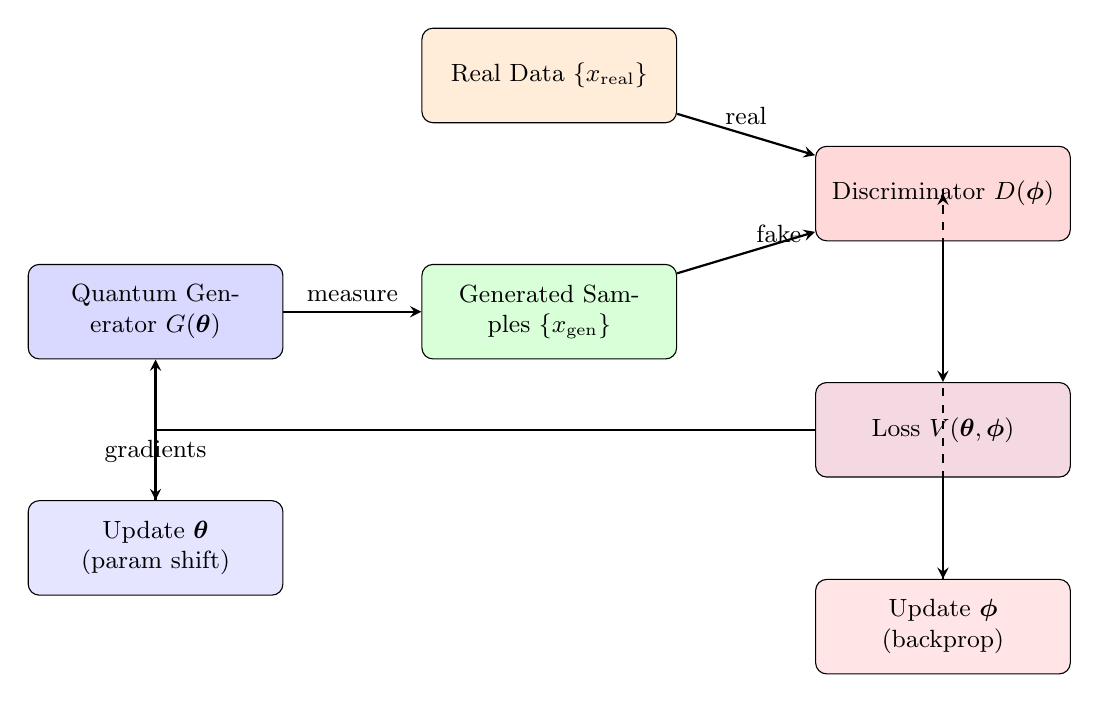
\begin{tikzpicture}[
    box/.style={draw, rounded corners, minimum width=3.2cm, minimum height=1.2cm, text width=3cm, align=center, font=\small},
    arrow/.style={->, thick, >=stealth},
    every node/.style={font=\small}
]

% Generator
\node[box, fill=blue!15] (gen) at (0, 0) {Quantum Generator $G(\boldsymbol{\theta})$};

% Samples
\node[box, fill=green!15] (gsamp) at (5, 0) {Generated Samples $\{x_{\text{gen}}\}$};

% Real data
\node[box, fill=orange!15] (real) at (5, 3) {Real Data $\{x_{\text{real}}\}$};

% Discriminator
\node[box, fill=red!15] (disc) at (10, 1.5) {Discriminator $D(\boldsymbol{\phi})$};

% Loss
\node[box, fill=purple!15] (loss) at (10, -1.5) {Loss $V(\boldsymbol{\theta}, \boldsymbol{\phi})$};

% Update G
\node[box, fill=blue!10] (updg) at (0, -3) {Update $\boldsymbol{\theta}$ (param shift)};

% Update D
\node[box, fill=red!10] (updd) at (10, -4) {Update $\boldsymbol{\phi}$ (backprop)};

% Arrows
\draw[arrow] (gen) -- (gsamp) node[midway, above] {measure};
\draw[arrow] (gsamp) -- (disc) node[midway, above right] {fake};
\draw[arrow] (real) -- (disc) node[midway, above] {real};
\draw[arrow] (disc) -- (loss);
\draw[arrow] (loss) -- (updd);
\draw[arrow] (loss) -| (updg) node[midway, below] {gradients};
\draw[arrow] (updg) -- (gen);
\draw[arrow, dashed] (updd) -- ++(0, 5.5) -| (disc);

\end{tikzpicture}
\end{center}

the dashed arrow shows the discriminator update feeding back into itself. the solid arrows show the main flow: generate samples, discriminate, compute loss, update both networks.

%% ========================================================
\section{Born Machine Sampling Concept}
%% ========================================================

lets visualize how a Born machine generates samples:

\begin{center}
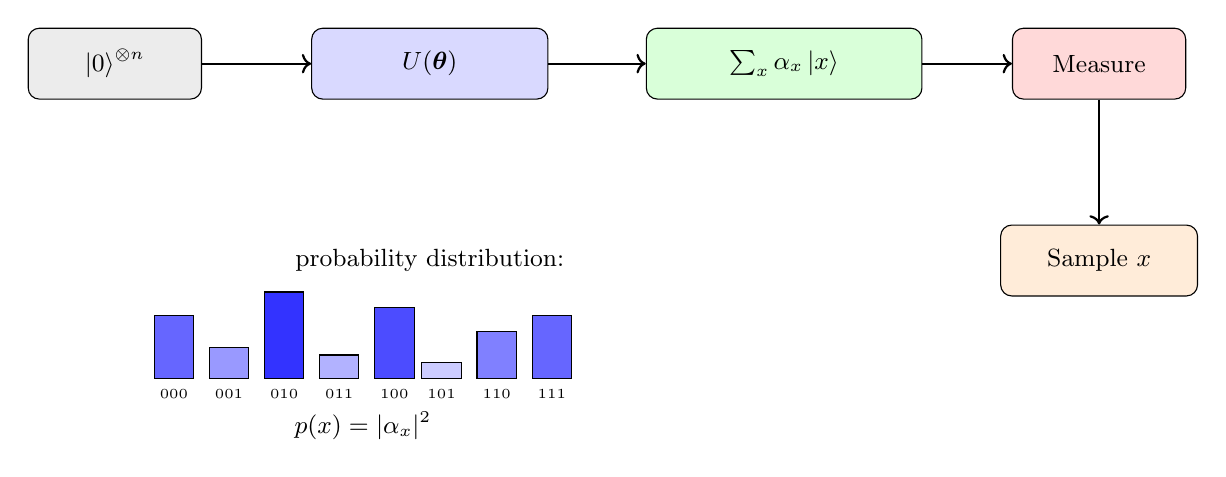
\begin{tikzpicture}[
    every node/.style={font=\small},
    box/.style={draw, rounded corners, minimum width=2.2cm, minimum height=0.9cm, align=center}
]

% Initial state
\node[box, fill=gray!15] (init) at (0, 0) {$\ket{0}^{\otimes n}$};

% Circuit
\node[box, fill=blue!15, minimum width=3cm] (circ) at (4, 0) {$U(\boldsymbol{\theta})$};

% Superposition state
\node[box, fill=green!15, minimum width=3.5cm] (super) at (8.5, 0) {$\sum_x \alpha_x \ket{x}$};

% Measurement
\node[box, fill=red!15] (meas) at (12.5, 0) {Measure};

% Output
\node[box, fill=orange!15, minimum width=2.5cm] (out) at (12.5, -2.5) {Sample $x$};

% Probability bars below
\node at (4, -2.5) {probability distribution:};

\draw[fill=blue!60] (0.5, -4) rectangle (1.0, -3.2);
\draw[fill=blue!40] (1.2, -4) rectangle (1.7, -3.6);
\draw[fill=blue!80] (1.9, -4) rectangle (2.4, -2.9);
\draw[fill=blue!30] (2.6, -4) rectangle (3.1, -3.7);
\draw[fill=blue!70] (3.3, -4) rectangle (3.8, -3.1);
\draw[fill=blue!20] (3.9, -4) rectangle (4.4, -3.8);
\draw[fill=blue!50] (4.6, -4) rectangle (5.1, -3.4);
\draw[fill=blue!60] (5.3, -4) rectangle (5.8, -3.2);

\node[font=\tiny] at (0.75, -4.2) {000};
\node[font=\tiny] at (1.45, -4.2) {001};
\node[font=\tiny] at (2.15, -4.2) {010};
\node[font=\tiny] at (2.85, -4.2) {011};
\node[font=\tiny] at (3.55, -4.2) {100};
\node[font=\tiny] at (4.15, -4.2) {101};
\node[font=\tiny] at (4.85, -4.2) {110};
\node[font=\tiny] at (5.55, -4.2) {111};

\node at (3.15, -4.6) {$p(x) = |\alpha_x|^2$};

% Arrows
\draw[->, thick] (init) -- (circ);
\draw[->, thick] (circ) -- (super);
\draw[->, thick] (super) -- (meas);
\draw[->, thick] (meas) -- (out);

\end{tikzpicture}
\end{center}

the circuit transforms $\ket{0}^{\otimes n}$ into a superposition, and measurement collapses it to a specific bitstring with probability given by the Born rule. by training the circuit parameters, we shape the probability distribution to match our target.

%% ========================================================
\section{Mode Collapse and Training Challenges}
%% ========================================================

training quantum generative models is hard. lets be honest about the challenges.

\subsection{Mode Collapse}

just like classical GANs, QGANs can suffer from mode collapse:

\begin{definition}[Mode Collapse]
mode collapse occurs when the generator learns to produce only a subset of the modes (peaks) in the target distribution, ignoring the rest. the generator gets ``stuck'' producing a few high-probability outcomes.
\end{definition}

in the quantum case, mode collapse means the circuit state has high amplitude on only a few computational basis states, even though the target distribution is more spread out.

causes in the quantum setting:
\begin{itemize}[nosep]
    \item limited circuit depth (not enough entanglement to represent multimodal distributions)
    \item barren plateaus making it hard to escape local minima
    \item discriminator overpowering the generator
\end{itemize}

\subsection{Shot Noise}

\begin{keypoint}
this is the uniquely quantum challenge: every probability estimate from a quantum circuit has statistical uncertainty from finite sampling (shot noise). if u use $S$ shots, the uncertainty in probability estimates is $O(1/\sqrt{S})$.
\end{keypoint}

this affects training in several ways:
\begin{itemize}[nosep]
    \item gradients r noisy: the parameter-shift rule requires estimating expectation values, each with shot noise
    \item the discriminator receives noisy samples, making its gradients noisy too
    \item for Wasserstein QGANs, the critic function must be estimated from noisy samples
\end{itemize}

the shot noise compounds with the usual stochastic gradient noise. in practice, u need $O(10^3 - 10^4)$ shots per circuit evaluation, and the parameter-shift rule doubles that (two circuit evaluations per gradient component).

total cost per training step: $O(P \cdot S)$ circuit evaluations, where $P$ is the number of parameters and $S$ is the number of shots. this adds up fast.

\subsection{Hardware Noise}

on real NISQ devices, gate errors, decoherence, and readout errors all distort the output distribution. this means the generator is effectively learning a noisy version of the target distribution, convolved with the hardware noise.

mitigation strategies:
\begin{itemize}[nosep]
    \item error mitigation techniques (zero-noise extrapolation, probabilistic error cancellation)
    \item noise-aware training (include a noise model in the optimization loop)
    \item using more robust loss functions (Wasserstein distance is more tolerant of noise than KL divergence)
\end{itemize}

\subsection{Barren Plateaus (Again)}

yes, barren plateaus strike again. for quantum generative models:
\begin{itemize}[nosep]
    \item random initialization of deep circuits leads to exponentially vanishing gradients
    \item the problem is worse for global loss functions (like fidelity between full quantum states)
    \item local loss functions (like MMD with local kernels) r more resistant
\end{itemize}

the standard mitigations apply: shallow circuits, structured initialization, local cost functions.

%% ========================================================
\section{Comparison: QBM vs QGAN vs Born Machine}
%% ========================================================

lets put it all together:

\begin{center}
\renewcommand{\arraystretch}{1.4}
\begin{tabular}{|p{3cm}|p{3.5cm}|p{3.5cm}|p{3.5cm}|}
\hline
\textbf{Property} & \textbf{QBM} & \textbf{QGAN} & \textbf{Born Machine} \\
\hline
model state & thermal state $e^{-\beta H}/Z$ & pure state from PQC & pure state from PQC \\
\hline
output type & mixed state (density matrix) & classical samples (after measurement) & classical samples (after measurement) \\
\hline
training signal & quantum relative entropy & adversarial (discriminator) & MMD or KL divergence \\
\hline
parameters & Hamiltonian couplings $J_{ij}, h_i, \Gamma_i$ & circuit rotations $\theta_k$ & circuit rotations $\theta_k$ \\
\hline
can represent mixed states & yes (naturally) & only via ancilla tracing & only via ancilla tracing \\
\hline
training difficulty & hard (need thermal state prep) & moderate (adversarial instability) & easiest (direct optimization) \\
\hline
key paper & amin et al. 2018 & zoufal et al. 2019 & liu and wang 2018 \\
\hline
best for & quantum data, thermal distributions & loading classical distributions & simple generative tasks \\
\hline
\end{tabular}
\end{center}

\begin{intuition}
if u want the simplest quantum generative model, use a Born machine. if u want to load a classical distribution into a quantum state (e.g., for quantum finance), use a QGAN. if u r working with genuinely quantum data (e.g., thermal states of physical systems), consider a QBM.
\end{intuition}

%% ========================================================
\section{Advanced Topics}
%% ========================================================

\subsection{Fully Quantum GANs}

in a fully quantum GAN, both the generator and discriminator r quantum circuits. the discriminator takes a quantum state as input (no intermediate measurement) and outputs a classification.

the loss function becomes:
\[
V = \mathrm{Tr}(D \cdot \rho_{\text{real}}) - \mathrm{Tr}(D \cdot \rho_{\text{gen}})
\]
where $D$ is a quantum observable (the ``discriminator operator'').

lloyd and weedbrook (2018) first proposed this. the advantage: the discriminator can detect quantum features (coherences, entanglement) that would be invisible to a classical discriminator working with measurement outcomes.

\subsection{Conditional QGANs}

just like classical conditional GANs, u can condition the quantum generator on a label or class:

\begin{center}
\begin{quantikz}
\lstick{$\ket{0}$} & \gate{R_Y(c_1)} & \ctrl{1} & \gate{R_Y(\theta_1)} & \ctrl{1} & \meter{} \\
\lstick{$\ket{0}$} & \gate{R_Y(c_2)} & \targ{} & \gate{R_Y(\theta_2)} & \targ{} & \meter{} \\
\lstick{$\ket{0}$} & \qw & \ctrl{1} & \gate{R_Y(\theta_3)} & \ctrl{1} & \meter{} \\
\lstick{$\ket{0}$} & \qw & \targ{} & \gate{R_Y(\theta_4)} & \targ{} & \meter{}
\end{quantikz}
\end{center}

here $c_1, c_2$ r determined by the conditioning variable (e.g., class label). the circuit generates samples from the class-conditional distribution.

\subsection{Quantum Wasserstein GAN}

chakrabarti et al. (2019) proposed a quantum version of WGAN where the critic is a quantum circuit. the Wasserstein distance between quantum states is:
\[
W(\rho, \sigma) = \max_{\|O\|_L \leq 1} |\mathrm{Tr}(O(\rho - \sigma))|
\]
where $\|O\|_L \leq 1$ means the observable $O$ has bounded Lipschitz norm. in practice, this is approximated by parameterizing $O$ as a PQC and adding a gradient penalty.

%% ========================================================
\section{Practical Considerations}
%% ========================================================

\subsection{How Many Qubits Do U Need?}

for a QGAN loading a distribution over $K$ values:
\[
n = \lceil \log_2 K \rceil \text{ qubits}
\]

so for a distribution over 256 values (e.g., 8-bit discretization), u need 8 qubits. for 1024 values, 10 qubits. this is modest by quantum computing standards, but remember that each additional qubit doubles the Hilbert space dimension.

\subsection{Circuit Depth vs Expressivity}

\begin{theorem}[Approximate Universality]
a hardware-efficient ansatz with $L$ layers of single-qubit rotations and entangling gates on $n$ qubits can approximate any $n$-qubit state to accuracy $\epsilon$ with:
\[
L = O\left(\frac{2^n}{n}\right)
\]
layers in the worst case. but for structured distributions (which is wt we typically care about), much fewer layers suffice.
\end{theorem}

in practice, zoufal et al. found that $L \sim 3n$ layers worked well for distributions on up to 5 qubits.

\subsection{Comparison with Classical Loading}

classical state preparation of an arbitrary $n$-qubit state requires $O(2^n)$ CNOT gates. the QGAN approach requires:
\begin{itemize}[nosep]
    \item training time: $O(T \cdot P \cdot S)$ circuit evaluations (T iterations, P parameters, S shots)
    \item inference time: $O(n \cdot L)$ gates per sample
\end{itemize}

if $n \cdot L \ll 2^n$ (which it is for reasonable $n$ and $L$), the QGAN approach wins at inference time. the training is expensive but is a one-time cost.

%% ========================================================
\section{Summary}
%% ========================================================

ok lets wrap up wt we covered:

\begin{enumerate}[label=\arabic*.]
    \item \textbf{classical foundations}: Boltzmann machines use energy-based models with contrastive divergence training. GANs use adversarial training with a minimax game.

    \item \textbf{quantum Boltzmann machines}: replace classical energy with quantum Hamiltonian. transverse field terms create quantum coherences that can represent correlations beyond classical BMs. training requires thermal state preparation, which is hard.

    \item \textbf{QGANs}: quantum generator (PQC) + classical or quantum discriminator. the main application is loading probability distributions into quantum states. zoufal et al. 2019 showed this works on real hardware.

    \item \textbf{Born machines}: the simplest quantum generative model. probability from the Born rule. trained with MMD or KL divergence. can represent exponentially complex distributions with polynomial parameters.

    \item \textbf{applications}: financial data loading (for quantum Monte Carlo), drug molecule generation, anomaly detection.

    \item \textbf{challenges}: mode collapse, shot noise, hardware noise, barren plateaus. training quantum generative models is harder than training quantum classifiers.
\end{enumerate}

the big picture: quantum generative models exploit the exponential dimensionality of Hilbert space to represent complex distributions compactly. the most practical near-term application is distribution loading for quantum algorithms. the field is young and theres a lot of room for new ideas.

next lecture: we step back and ask the big questions --- wt is the actual power of QML? where is quantum advantage proven, and where is it just hoped for? we'll also wrap up the course.

%% ========================================================
\section{Further Reading}
%% ========================================================

\begin{enumerate}[label={[\arabic*]}]
    \item zoufal, lucchi, woerner. ``quantum generative adversarial networks for learning and loading random distributions.'' npj Quantum Information, 2019.
    \item liu, wang. ``differentiable learning of quantum circuit Born machines.'' Physical Review A, 2018.
    \item amin, andriyash, rolfe, kulchytskyy, melko. ``quantum Boltzmann machine.'' Physical Review X, 2018.
    \item lloyd, weedbrook. ``quantum generative adversarial learning.'' Physical Review Letters, 2018.
    \item chakrabarti, huang, musser, et al. ``quantum Wasserstein generative adversarial networks.'' NeurIPS, 2019.
    \item goodfellow et al. ``generative adversarial nets.'' NeurIPS, 2014.
    \item hinton. ``training products of experts by minimizing contrastive divergence.'' Neural Computation, 2002.
\end{enumerate}

\end{document}
